\documentclass[11pt,twoside,a4paper]{book}

\usepackage[british]{babel}   % use UK hyphenation, etc.
\usepackage[T1]{fontenc}      % font printing stuff
\usepackage{ae,aecompl}       % scalable, non-bitmap fonts
\usepackage[pdftex]{graphicx} % enables graphics for pdf-latex
\usepackage{color}            % enables use of colour for text
\usepackage{subfig}           % enables subfigures
\usepackage{amsmath}          % the one and only AMS-Math
\usepackage{makeidx}          % creating an index

% ----------------------------------------------------------
% My own commands
% ----------------------------------------------------------
\newcommand{\mynote}[1]{\emph{\textbf{\textcolor{red}{#1}}}}
\newcommand{\ra}{$\rightarrow$}
\newcommand{\cmd}[1]{\texttt{#1}}
\newcommand{\ogs}{OpenGeoSys }
\newcommand{\bstart}[1]{\noindent\textbf{#1} }
\newcommand{\degree}{\ensuremath{^\circ}}


% ----------------------------------------------------------
% Typography
% ----------------------------------------------------------
\nonfrenchspacing             % grosser Abstand nach Satzende
\widowpenalty 10000           % Keine Hurenkinder
\displaywidowpenalty 10000    % Keine Hurenkinder (Formeln)
\clubpenalty 10000            % Keine Schusterjungen


% ----------------------------------------------------------
% Headers
% ----------------------------------------------------------
\usepackage{fancyhdr}         % formating page headers

\renewcommand{\headrulewidth}{0.4pt}
\renewcommand{\footrulewidth}{0pt}
\fancyhead{} \fancyfoot{}
\fancyhead[RE]{The OpenGeoSys Data Explorer}
%\fancyhead[RE]{\nouppercase{\leftmark}}
\fancyhead[LO]{\nouppercase{\leftmark}}
\fancyhead[LE,RO]{\thepage}


% ----------------------------------------------------------
% Hyperref Options
% MUSS AM SCHLUSS DER PRAEAMBEL STEHEN!
% ----------------------------------------------------------
\usepackage{hyperref}         % references and links within the document

\hypersetup{
  pdftitle={OGS Data Explorer - User Manual},
  pdfsubject={Manual},
  pdfauthor={Karsten Rink},
  pdfcreator={LaTeX2e},
  plainpages=false,           % For problems with page referencing
  hypertexnames=false,        % For handling subfigures correctly
  bookmarks=true,             % I want bookmarks
  bookmarksnumbered=false,    % Include the section numbers in the list
  bookmarksopen=true,         % In the list, display highest level only
  bookmarksopenlevel=3,       % Display three levels of bookmarks
  pdfpagemode=UseNone,        % Fit screen (or "`FullScreen"')
  pdfstartview=Fit,
  pdfborder=0,                % I don't want those silly boxes
  breaklinks=true,            % Allow breaks in links
  colorlinks=false            % Don't change coloring of links
}


% ----------------------------------------------------------
% Document description
% ----------------------------------------------------------
\title{{\LARGE OpenGeoSys Data Explorer}\\[0.5em] Manual}
\author{Karsten Rink}
\graphicspath{{pics/}}
\setlength{\fboxsep}{0mm}
\linespread{1.10}

\makeindex

\hyphenation{know-ledge}

% ----------------------------------------------------------
% Start of document
% ----------------------------------------------------------
\begin{document}

\pagestyle{empty}
\maketitle
\newpage

\vspace*{12cm}
\begin{tabbing}
\hspace*{6cm}\=aa\kill
\begin{minipage}[t]{0.62\textwidth}
\noindent This manual has been compiled based on the \ogs Data Explorer 5.3 \\
(released on 25 April 2012).\\
\\
This document as well as its sources are published under Creative Commons Attribution-Noncommercial-Share Alike 3.0 Un\-por\-ted License. For more information go to \url{http://creativecommons.org/licenses/by-nc-sa/3.0/}. \\
\\
\noindent Special thanks to Lars Bilke and Thomas Fischer and everyone else helping with the development of the software.
\end{minipage}
\> \\
\end{tabbing}

\newpage

\tableofcontents

\cleardoublepage

\pagestyle{fancy}

\chapter{Introduction}

This manual has been written to give a quick overview over the functionality of the \ogs Data Explorer. Existing functionality is explained and typical workflows are detailed step by step.

\bigskip

\ogs (formerly Rockflow) is a programme for the simulation of (coupled) thermal, hydrological, mechanical and chemical processes. Over various iterations the software is about $20$ years old and compiles a large amount of functionality, interfaces and numerical solvers. It is, however, a command line tool. Therefore, it is difficult to get a feeling for the data that is handled by the programme and simulation results cannot be directly verified without the help of other tools.

The \ogs Data Explorer is a graphical user interface (GUI) has been developed to fill that gap and provides a means for the visualisation of data. It employs the same basic data structures as the command line tool and thus complements \ogs by giving the user a way to visually assess the data and see possible errors, inconsistencies or missing information.

However, it is important to keep in mind that the \ogs Data Explorer is \emph{not} a fully developed tool with a defined scope of functionality. Features are constantly being added and while everyone is making an effort to keep things as straightforward and robust as possible, it can be difficult to find out what the programme is currently capable of and how exactly things need to be done.

This manual will give you an overview of the features of the programme, how things work and what possible problems you might encounter. For more information on \ogs itself check out the OGS-Wiki\footnote{https://svn.ufz.de/ogs}.\index{OGS Wiki}

It is also highly recommended to always use the latest version of \ogs which is available on the Jenkins\footnote{http://jenkins-ci.org/} Build Server\footnote{https://svn.ufz.de/jenkins/}\index{Jenkins Build Server}.

\subsection*{Important concepts}

\begin{figure}[tb]
\begin{center}
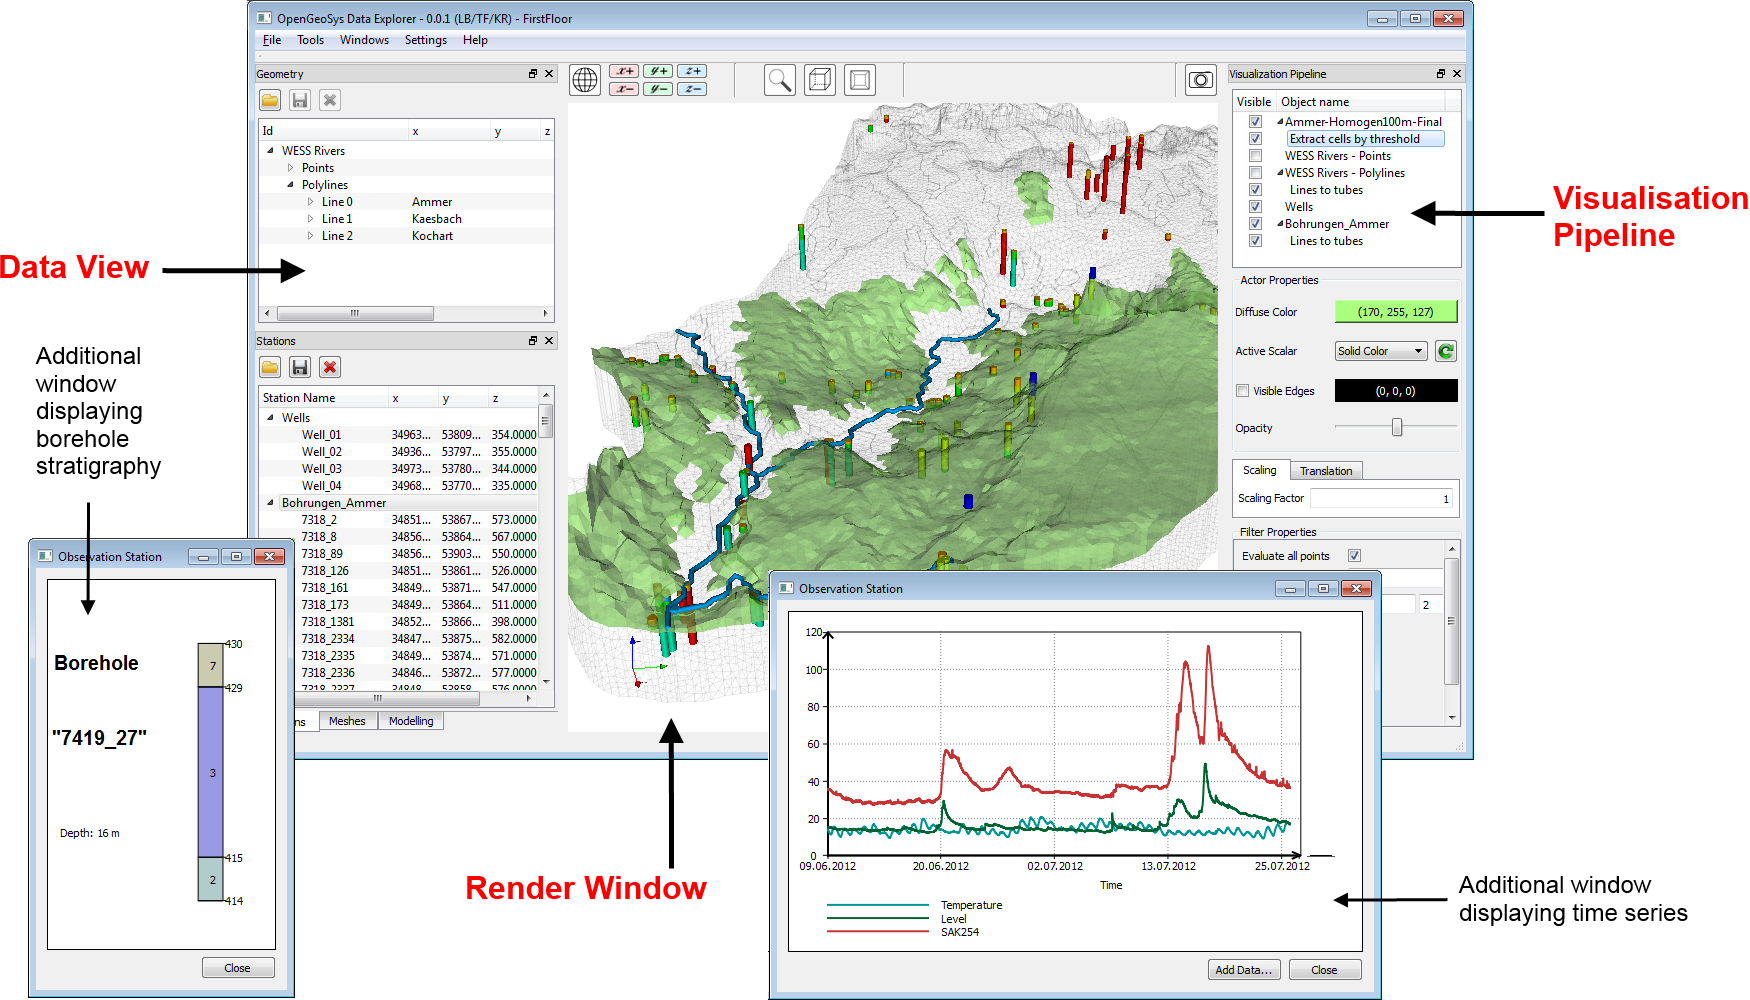
\includegraphics[width=0.99\linewidth]{gui}
\caption{The graphical user interface of the \ogs Data Explorer.}
\label{fig:gui}
\end{center}
\end{figure}

Within this manual a number of terms will appear over and over and it is important to know what they mean, to be able to follow the instructions.

Figure \ref{fig:gui} shows a screenshot of the GUI of the \ogs Data Explorer. The three basic parts of the user interface are marked as ``Data View'', ``Render Window'' and ``Visualisation Pipeline''. These elements and the information they contain are explained in detail in section \ref{datavisualisation} and these names will pop up again and again in this manual so it is important to recognise which parts of the graphical user interface they specify. Additional windows might pop up from time to time for data that is not suitable for 3D visualisation, such as time series sensor data or borehole stratigraphies. 

\ogs is written in the C++ programming language. As many other programming languages it allows the developer to add so called libraries that define a certain set of functionality. This means a programmer does not need to implement every function provided by a programme himself but instead can depend on functionality provided by the library. The Data Explorer makes use of a number of such libraries. The two most important ones are called Qt\footnote{http://qt.nokia.com} and VTK\footnote{http://www.vtk.org}. 

Qt\index{Qt} is a library mainly providing functionality for a user interface, i.e. the definition of windows, dialogues and everything you expect to see in there, such as buttons, lists, menus, etc. Qt offers a lot more than that but explaining it all would go beyond the scope of this manual. Elements of the Data Explorer that make use of Qt are for instance the ``Data View'' or the windows displaying diagrams or borehole stratigraphies.

VTK\index{VTK} (``\textbf{V}isualisation \textbf{T}ool\textbf{k}it'') is a graphics library which can be employed for the visualisation of objects in 3D. It also includes functionality to read and write these 3D objects from and to files. These ``VTK-files'' and can also be used by the Data Explorer but also by any other programme supporting VTK, such as ParaView\footnote{http://www.paraview.org}\index{ParaView} or OpenFOAM\footnote{http://www.openfoam.com}\index{OpenFOAM}. The ``Render Window'' of the Data Explorer and anything that is displayed within has been constructed using VTK.



\chapter{Working with the Data Explorer}

\section{Loading data...}

\subsection{Native File Formats}
\label{nativefileformats}
\index{File formats}

\ogs has a large number of native file formats for storing geometrical data (*.gli), meshes (*.msh), processes (*.pcs), FEM conditions (such as boundary conditions (*.bc)) and material properties (e.g. fluid properties (*.mfp)) and many more.

Not all of them can be loaded into the user interface since not all of them contain data that can be visualised. Things are additionally made difficult as the file standards for the programm are currently changed from GeoSys4 ASCII files to OGS XML files\footnote{http://www.w3.org/XML/}. For this reason there exists -- at least at the time of this writing -- two file standards for certain kinds of data. Hopefully, this unfortunate situation is resolved soon.

You can open native OGS files by clicking \cmd{File\ra Open...}\index{Loading geometry}\index{Loading meshes}.

Supported native files in GeoSys4 \textbf{ASCII} format are:
\begin{itemize}
\item Geometry (*.gli)\index{Geometry}\\
    Containing geometrical data such as points, polylines and surfaces (in this file format surfaces are defined by closed polylines and are therefore always describing planes).
\item Meshes (*.msh)\index{Meshes}\\
    Domain discretisation in 2D or 3D. Each mesh contains a set of nodes (points) as well as a set of elements defined by a subset of these nodes. A mesh may contain different kinds of elements. OGS supports the following element types\index{Element types}: lines, triangles, quadrilaterals, tetrahedra, hexahedra, pyramids, prisms.\\
    Meshes may be classified into structured or unstructured meshes. Note, that \ogs treats all meshes as unstructured.
\item FEM Conditions (*.bc, *.ic, *.st): Containing boundary conditions, initial conditions and source terms, respectively. These files contain information that links phenomena with a given set of values (or distribution of values) to geometric objects or mesh nodes.
\end{itemize}

Supported OGS \textbf{XML} file formats are:
\begin{itemize}
\item Geometry files (*.gml)\\
    Containing geometrical data such as points, polylines and surfaces (in this file format surfaces are triangulated and can therefore describe any kind of surface).
\item Observation sites (*.stn) \index{Stations}\index{Boreholes}\\
    XML file format containing information for observation stations as well as boreholes. The files also describe points in space but with additional information (such as stratigraphic information for boreholes). Also, this data is visualised in a different way.
\item FEM Conditions (*.cnd): Containing boundary conditions, initial conditions and source terms needed for simulation of processes. These files contain information that links phenomena with a given set of values (or distribution of values) to geometric objects or mesh nodes.
\item \ogs project files (*.gsp)\index{Project files}\\
    XML file format for \ogs projects. These files contain files related to a given project. All of these files will be loaded upon loading the *.gsp file. This is especially useful for projects consisting of a large number of input files.
\end{itemize}

\subsubsection{Additional Information about Loading FEM Conditions}
\index{Loading FEM conditions}

Besides loading FEM Conditions via  \cmd{File\ra Open...}, it is also possible to right-click on any geometry in the data view to assign FEM conditions to a geometry via \cmd{Load FEM Condition...}. Upon loading it is checked if a corresponding geometry for these conditions is available. For XML-files the associated geometry name is saved in the cnd-file, for old file types it is simply assumed that the geometry name will be the same as the name of the condition-file. If no geometry of this name is found, the data will not be loaded. You may may also add source terms of the process distribution ``DIRECT'' directly on meshes nodes (again, via right-clicking on a mesh) and the conditions will then be displayed on the respective mesh nodes defined in the input file.

For the visualisation, the correct scalar values in the render window will currently only be displayed for process distribution types ``CONSTANT'', ``LINEAR'' and ``DIRECT''.\footnote{For an overview over what process distribution types are, which types are supported by the system and how they influence a subsequent simulation please refer to technical documentation of \ogs.}

\subsubsection{Conversion of Native Files}
\index{OGS File Converter}

It is possible to convert data between GeoSys4 ASCII files and \ogs XML files (and vice versa) via the \emph{OpenGeoSys File Converter}. The file converter can be called from \cmd{Tools\ra File Converter...} and is also available as a stand-alone tool upon download of \ogs. Simply select which type of file you would like to convert, specify file names and press okay.

The file converter currently supports conversion of geometry and FEM condition files, but will be extended in the future as file formats are changed to XML.

\subsection{Import File Formats}
\label{Import File Formats}
\index{Import file formats}

\begin{figure}[tb]
\begin{center}
\includegraphics[width=0.99\linewidth]{interfaces}
\caption{Supported file formats for import and export of data.}
\label{fig:interfaces}
\end{center}
\end{figure}

A number of non-native file formats can also be loaded and visualised in the Data Explorer. To import these files click on \cmd{File \ra Import Files} and select the appropriate entry.

Depending of which file format you want to load, quality of the interface varies depending on a number of facts such as if the file format is an open standard or if there were enough input files to test the interface when it was implemented.

Currently the following file formats are supported:
\begin{itemize}
\item ESRI \textbf{shape} files (*.shp)\index{Shape files}\\
Vector files specifying points, polylines and polygons. The interface for shape files is thoroughly tested and there should be no problems whatsoever. However, note that a lot shape files come with a database file containing additional information (*.dbf) which has no standardised table structure and therefore is not analysed or imported by the data explorer.
\item Aquaveo \textbf{GMS} files (*.txt, *.3dm)\index{GMS files}\\
Text or mesh files specifying boreholes (*.txt) or layered meshes build from tetrahedrons and prisms. This interface has been tested with number of cases and should work fine.
\item \textbf{GMSH} files (*.msh)\index{GMSH files}\\
Mesh files containing unstructured grids. As an exception these files are \emph{not} loaded via the import menu but you have to load them directly via \cmd{File\ra Open...}. The interface should work perfectly however.
\item \textbf{GoCAD} files (*.ts)\index{GoCAD files}\\
This interface is in an unfinished state. However, there exists a programming interface to write OGS-files directly from GoCAD. Please talk to the development team if you need to load data into OGS.
\item \textbf{NetCDF} files (*.nc, *.cdf)\index{NetCDF files}\\
A machine-independent format that contains all kinds array-oriented scientific data. The interface only works from GUI as it requires to open a dialogue where data dimensions and time steps need to specified. The netCDF date will then be converted into either a mesh or a raster. Conversion into a mesh allows to set more parameters such as the requested mesh element type and the data representation (also see section \ref{meshraster}).
\item \textbf{FEFLOW} files\index{FEFLOW files}\\
Allows the import FEFLOW problem ASCII files (*.fem). This interface imports only geometry, e.g. polygons, and meshes.
\item \textbf{Petrel} files\index{Petrel files}\\
This interface is in an unfinished state. Please talk to the development team if you need to load data into OGS.
\item \textbf{Raster} files (*.asc, *.bmp, *.jpg, *.grd *.png, *.tif)\index{Raster files}\index{Images}\\
Image data files that may contain satellite images, etc. ESRI and Surfer ASCII raster files (*.asc / *.grd) as well as GeoTIFF (*.tif) files contain geo-referenced data, while common image files (*.bmp, *.jpg, *.png) do not. This interface should work for all supported file types although it can be quite slow for large raster files.
\item \textbf{TetGen} files\index{TetGen files}\\
Allows the import files created with the TetGen mesh generator. This interface currently only reads the node- and tetrahedra-files created by the software (i.e. *.node and *.ele).
\item Visual Toolkit (\textbf{VTK}) files (*.vti, *.vtk, *.vtp, *.vtr, *.vts, *.vtu)\index{VTK files}\\
Files containing data for graphic objects, ranging from image files (*.vti) to structured (*.vts) or unstructured meshes (*.vtu). All data sets may include additional data in the form of scalar arrays. This interface should work perfectly.
\end{itemize}

\subsection{Removal of Data}
\index{Removing data}

You can remove all data loaded into \ogs by right-clicking the data set in its respective data view and selected \cmd{Remove data}. Specifically you can also remove only polylines or surfaces only from a geometry. The only exception to this rule are geometric points which can only be removed if both surfaces and polylines are already deleted as both kinds of objects are dependent on points. Regardless of the previous remarks you can also remove geometries as whole.

\section{Data Visualisation}
\label{datavisualisation}

Technically, data (or a representation thereof) loaded into the programme is displayed at three different locations (see figure \ref{fig:gui}):

\subsection{Data Views}
\index{DataView}

There are four different DataView-Tabs in the programme where the data is visible in the form of lists. Which of the tabs is used depends on the data. There is one tab for geometrical information, one for meshes, one for stations (i.e. observation sites) and one for modelling information (i.e. processes, boundary conditions, etc.)

The DataView for geometrical information contains a list of geometries. Each geometry-item has up to three children titled ``Points'', ``Polylines'' and ``Surfaces'' containing the information about the respective geometrical objects. For example, the item `Points' contains a list of points and for each item (i.e. each point) its index, the coordinates and (if existing) the name of the object can be displayed. Each geometry \emph{needs} to contain a list of points. Other geometrical objects (i.e. polylines or surfaces) are optional. Upon selecting a geometrical object in the DataView, the object will also be highlighted\index{Highlighting objects} in the render window. For better visibility a point will be marked by a small ball, a line by a tube.

Note, that the mesh-tab is subdivided into a view of the meshes loaded into the programme (and the elements contained within each mesh) and a second window called ``Element Properties''. If you pick any element from the render window, all available information concerning that element (such as nodes, volume, element type, etc.) will be displayed here. For more information on how to pick mesh elements, see the next section.

\subsection{Render Window}
\index{Render window}

\begin{figure}[tb]
\begin{center}
\subfloat{\includegraphics[width=0.48\linewidth]{error1}}\enspace
\subfloat{\includegraphics[width=0.48\linewidth]{error2}}
\end{center}
\caption{Examples for inconsistencies within the data. The left image show inconsistencies between two meshes. The right images show a number of boreholes, one of which has a wrong offset.} \label{fig:error}
\end{figure}

The render window is the part of the GUI where all the data is visualised in a user-controlled 3D scene. The process of ``drawing'' an object in the render window is technically called the \emph{rendering} of the object and will be referred to as such in the following. The render window is where you can actually see your data as well as the effects of all the changes you do somewhere else in the programm or in the input files.

One of the big advantages of the Data Explorer is in the fact that this visual inspection of the data also allows you to assess your data and to find inconsistencies and errors. Figure \ref{fig:error} gives examples of such inconsistencies.

You can manipulate the 3d view by using the mouse. Holding the left mouse button and moving the mouse will rotate\index{Rotating} everything around the focal point of the scene (by default this is the center point of your data). By holding the middle mouse button you can pan the view which means you translate\index{Translation} left / right and up / down. By holding the right mouse button or moving the mouse wheel you can zoom\index{Zooming} in and out.

There is alternative mouse button functionality assignment which is activated by holding the Spacebar. When activated, left clicks pick\index{Picking} a cell of the actually selected visualisation pipeline object. This allows to mark a certain cell of the visualisation, such as the selection of a mesh element for displaying information related to that element. On right clicking the picked position is set as the focal point of the camera. This is useful for a better examination of an interesting region of the data so with focal point set to that region you can easily rotate and zoom around.

You can deselect the cell by holding Spacebar and clicking somewhere into the background of the render window.

\bigskip

Note, that you can make screenshots\index{Screenshots} of the content of the render window at any time. Simply press the \cmd{Screenshot}-button located above the render window and a small dialogue will open that allows you to select the scaling factor of the image. This is useful for creating large image (e.g. for posters) without artefacts.

\subsection{Visualization Pipeline}
\index{Visualization pipeline}

The visualisation pipeline looks very similar to the data views described above. However, the items displayed in this tab are a list of the graphical objects displayed (rendered) in the render window. For further reference these will be called \emph{visualisation items}. Each visualisation item has a checkbox beside its name that determines if the object is displayed in the render window or not. You can check or uncheck this box at any time, no data is lost if you uncheck it.

The relationship between data views, visualisation pipeline and render window is not completely straightforward without knowing the internal data structures of the programme but the basic concept is this:

For each data set loaded into the programme one or more visualisation items are created and then displayed in the render window. In most cases the relationship is not that difficult to understand: If a mesh is loaded, a new visualisation item is created and displayed in the render window. If a list of observation sites is loaded, again one visualisation item is created that represents the graphical object displayed in the render window. While you can expand that list of stations in the data view and see information about each station contained in the list, the visualisation item cannot be expanded. It is a substitute for the visualisation of said list in the render window. In the same vain, if a geometry is loaded into the programme up to \emph{three} visualisation objects are created: one for the list of points, one for the list of polylines and one for the list of surfaces (depending on the existence of polylines and surfaces).

Section \ref{filters} explains how you can employ the visualisation pipeline to apply filters the visualisation items. These filters allow changes of the way each object is visualised and they are quite handy to show certain aspects of the data.

\section{Writing Data...}
\index{Saving data}

\subsection{Native Files}
You can save geometries, observation sites and meshes by right-clicking them in the Data View and selecting \cmd{Save data...}. You can also save all loaded data files by saving an \ogs project. Select \cmd{File\ra Save as...} and specify a project name. This option will save all geometries in *.gml files, all mesh meshes in *.msh files and all observation sites in *.stn files. Additionally it will create a project file (*.gsp). When loading the gsp-file later on it will also load the respective geometries and observation sites again. (Note: Other file formats -- e.g. for boundary conditions or processes -- will be added in the future)

\subsection{Export to Other Formats}
\index{Export formats}

Any geometric data loaded into \ogs can be exported into a GMSH *.geo file via \cmd{File\ra Save as...} and selecting ``GMSH gemetry files'' as the output format. Note, that this will merge all geometries loaded into the programme and that it will also save station-data as points (i.e. you lose any additional information associated with these stations). Before saving, the geometric information will be inserted into a quad tree structure to analyse the data and insert additional points (so-called `Steiner Points') at locations where not enough information for generation of a suitable mesh exists. This ensures the creation of an adequate result when meshing the geo-file within GMSH.\footnote{Note that this allows you to export any combination of data into GMSH format for subsequent meshing. The functionality described in section \ref{meshcreation} for meshing of data within \ogs requires a ``bounding polygon'' that serves as outer boundary of all the data contained within the mesh.}

\bigskip

You can also export data from \ogs into a number of graphics formats. This can be done for selected graphical objects by right-clicking the respective object in the visualisation pipeline and than select the desired format (VTK or OpenSG). Details on this can be found in section \ref{specvisoptions}.

You can also export the complete scene into the graphic formats VTK, OpenSG or VRML format. To do this select \cmd{File\ra Export\ra Format}. 

\chapter{Data Manipulation}

\section{Manipulating Geometrical Data}
\index{Manipulating geometrical data}

There is a small number of function to manipulate geometric data in \ogs. The common approach to the manipulation of \ogs input data is that it should be changed in a GIS or other specialised software of the user's choice which usually offers much more functionality for these things than \ogs ever could.

However, it is possible to set or change names for any geometrical object by right-clicking on the object and selecting \cmd{Set name...}\index{Setting names}\index{Changing names}. Upon saving the data again, the new or modified names will be saved in the corresponding file.

\subsubsection{Removing Duplicate Points}
\index{Removing geometric points}

Upon loading geometric data, the programme will check if any two geometric points are identical or \emph{almost} identical (within a small $\varepsilon$-range) and remove these points. GIS software often produces feature files that contain duplicate points which is not a problem within GIS but leads to all kinds of problems during tessellation of polygons or volumes as well as during a subsequent FEM simulation.

While the software will remove these duplicate points everytime a specific data set is loaded, it makes sense to save the cleaned data set and thus save loading time later on and be sure to work with a more suitable data set.

\bigskip
 
All other functions for manipulating geometry are associated with polylines and can be applied by right-clicking the ``Polylines'' item of any geometry in the Data View and then selecting \cmd{Connect Polylines...}.

\subsubsection{Connecting Polylines}
\index{Connecting polylines}
This function connects all the selected polylines to a single new polyline provided that the start- and end points of all segments are within the given maximum distance. The default maximum distance is $0.0$, meaning that start- and end points have to be identical. A name may be added to the resulting new polyline.

Note that if more than two start/end points are located within the given maximum distance, still only two of those points are connected. These points are chosen randomly. It is not advised to use a maximum distance that may lead to ambiguous results.

The newly created polyline is added to the geometry. All the polylines that are parts of this new line are still kept within the geometry.

\subsubsection{Creating Polygons by Closing Polylines}
\index{Creating polygons from polylines}
This function closes a (connected) polyline. Simply check `Close connected Polyline'. Again, if a name has been entered, this name will be assigned to the closed polyline.

\subsubsection{Creating Surfaces by Triangulating Polygons}
\index{Creating surfaces from polygons}
This function additionally creates a new surface by triangulating the newly created polygon. This simply requires checking `Create Surface from Polyline'. The newly created polyline has to be closed for that function to work. If a name has been entered, this name will be assigned to the surface.


\section{Time Series and Stratigraphic Data to Observation Sites}
\index{Time series data}\index{Stratigraphic data}

For observation sites within the ``Stations'' Data View it is possible to display additional information such as logger data at the site or the stratigraphy at a borehole.

To view the additional information of an observation site load a stn-file into the programme and right-click on any observation site in the data view. You will see either the menu entry ``View Stratigraphy...'' for a borehole or ``View Diagram...'' for a station. While a borehole will always have strategraphic data (at least one layer over its whole length), not all stations will have time series data attached (this needs to be specified in the input file). If such data exists, a dialogue will open which allows to set a few parameters: A start and end date are set based on the data in the attached time series file for this station. This date can be changed to only display a subset of the data. There are also checkboxes for all all time series contained in the file which allow to specifically select only the time series the user wants to see. Upon pressing OK a new window will open, displaying the requested information.

\section{Generating and Manipulating Meshes}

\subsection{Creating Meshes from Geometry}
\label{meshcreation}\index{Creating meshes}

By selecting \cmd{Tools\ra Mesh Generation...} a dialogue that allows the user to create meshes using information currently present in the programme. For this to work, the open-source mesh generating software GMSH\footnote{http://geuz.org/gmsh/} needs to be installed and be available from the location of the Data Explorer (i.e. located in the same directory or findable, e.g. via PATH-variable under MS Windows).

The user can select any geometry and observation sites that should be considered for generating the mesh. It is necessary that at least on polyline in any of the selected geometries is closed (i.e. is a polygon) and will serve as an outer boundary to the resulting mesh. Any further polygons found in the geometry will be meshed, polygons within polygons will simply be integrated within the encompassing larger shape. Note that all points of every data set considered for mesh generation and located within the outer boundary will be included as nodes in the final mesh. Therefore it makes sense to check if consecutive points of polylines are unnecessarily close together or too far apart.

Upon pressing \cmd{OK} a geometry-file (*.geo) for GMSH is written, GMSH is called to create the mesh and the newly created mesh is at once imported in the \ogs-Data Explorer. If not specified otherwise, the geo-file will be deleted again after the mesh has been created.

There is an \cmd{Advanced}-Tab in this dialogue that allows to set a number of parameters for the mesh. Most importantly, it can be chosen, if the new mesh should be adaptive or homogeneous. An adaptive mesh{Adaptive Meshes} is refined towards points or lines specified in the geometry while a homogeneous mesh has elements of roughly the same size everywhere in the domain (see figure \ref{fig:meshing}).

\begin{figure}[tb]
\begin{center}
\subfloat[Geometry]{\includegraphics[width=0.3\linewidth]{meshing-geo}\label{meshing-geo}}\enspace
\subfloat[Homogeneous mesh]{\includegraphics[width=0.3\linewidth]{meshing-hmg}\label{meshing-hmg}}\enspace
\subfloat[Adaptive mesh]{\includegraphics[width=0.3\linewidth]{meshing-adp}\label{meshing-adp}}
\end{center}
\caption{Meshing using geometric data and observation sites.} \label{fig:meshing}
\end{figure}

The specific parameters for adaptive meshes are:
\index{Adaptive meshes}
\begin{itemize}
\item \textbf{Max. number of points in Quadtree leaf:} Generally speaking, the smaller this number the more refined the resulting mesh will be. \\
    To give a more detailed explanation, basic knowledge about \emph{quad tree} data structures \footnote{http://en.wikipedia.org/wiki/Quadtree} is necessary: A tree structure is constructed by a sequential subdivision of the domain based on the distribution of relevant points in space. The criterium if a segment compromising a leaf is further refined is dependent on the number of points located within that segment. The size of the parameter relates to the maximum allowed size of mesh elements and additional points (\emph{Steiner points}) will be added to the data set to ensure the a certain refinement is guaranteed anywhere within the domain. Therefore, larger numbers of that parameters will usually result in coarser meshes while smaller numbers will result in finer meshes. \emph{Note that this is technically not a correct explanation as results are heavily dependent on how many points are located in certain sub-divisions of the domain, the existence of point clusters, etc.} See figure \ref{fig:quadtree} for an example.
\item \textbf{Mesh density scaling for points:} This is a scaling factor for the above parameter allowing for a refinement towards points located within the outer boundary. Again, smaller values will result in finer meshes.
\item \textbf{Mesh density scaling for stations:} This is exactly the same kind of scaling factor as for the option above, only for refinement towards observation sites, allowing a different mesh density for different regions of the mesh.
\end{itemize}

\begin{figure}[tb]
\begin{center}
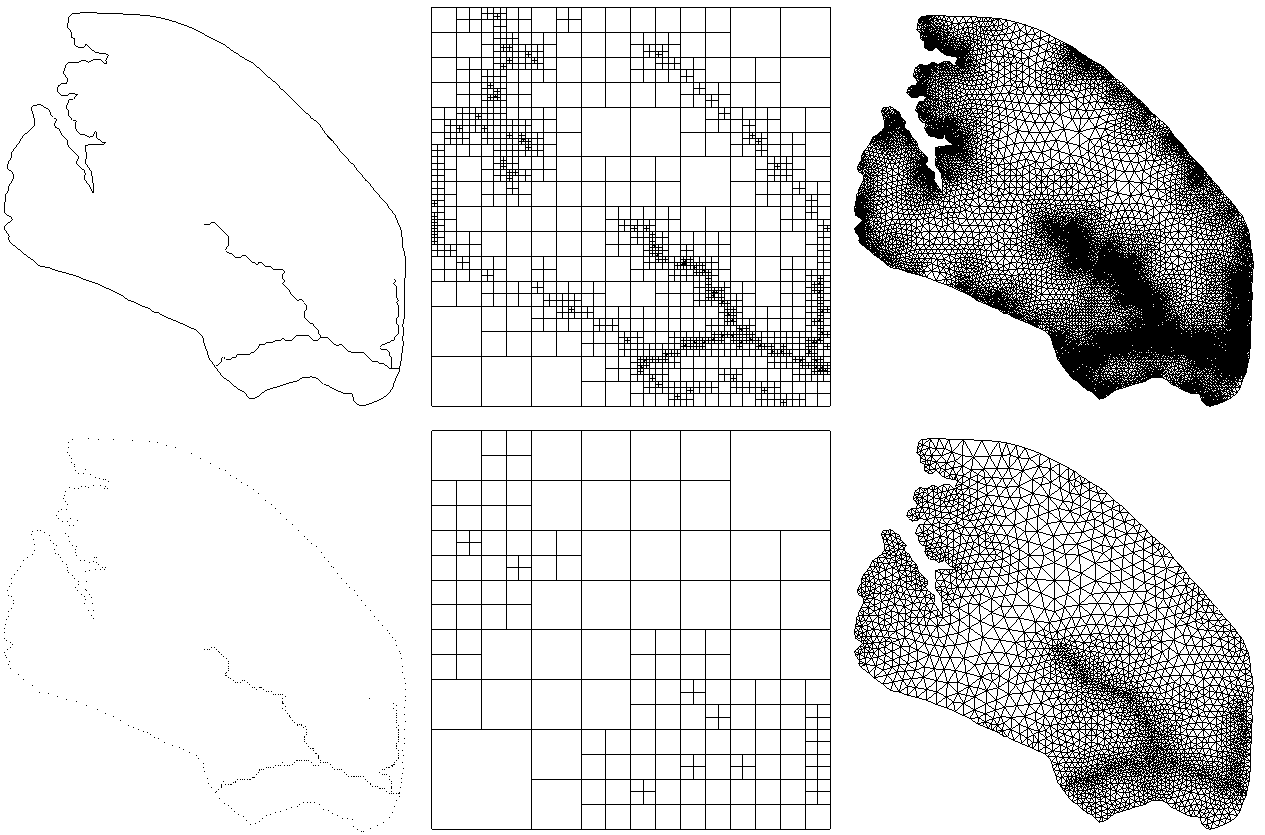
\includegraphics[width=0.95\linewidth]{quadtree}\label{quadtree}
\end{center}
\caption{Adaptive meshing of geometry. The left column depicts polyline and points that need to be meshed. In the middle the resulting quad trees can be seen, the upper on generated with a maximum of two points per leaf, the lower one with 10 points per leaf. The resulting meshes are shown on the right side. Notice that regions where no information is available have roughly the same element size while elements where point information is given differ vastly in element size.} \label{fig:quadtree}
\end{figure}

Likewise, you can select an \textbf{element size}\index{Element size} for homogeneous meshes.\index{Homogeneous meshes} Here, too, a smaller number will result in a finer mesh, as the value specifies the maximum edge length of mesh elements.

\bigskip

Default parameters for all options are already predefined and have worked well with most examples that have been tested. However, results are heavily dependent an the bounding box of all data sets used for mesh generation. Often it is necessary to play around with these numbers a bit. Usually it makes sense to start with larger parameters that result in coarser meshes to get a rough idea what the final mesh will look like and where potential problems may be located.

\subsection{Creating Meshes from Raster Files}
\label{meshraster}\index{Creating meshes}

\begin{figure}[tb]
\begin{center}
\subfloat[Raster]{\includegraphics[width=0.3\linewidth]{rastermesh1}\label{rastermesh1}}\enspace
\subfloat[Elevation]{\includegraphics[width=0.3\linewidth]{rastermesh2}\label{rastermesh2}}\enspace
\subfloat[Materials]{\includegraphics[width=0.3\linewidth]{rastermesh3}\label{rastermesh3}}
\end{center}
\caption{Creating meshes from raster files: Pixels can be either represented as a set of two triangles (Fig. \ref{rastermesh2}) or a square (Fig. \ref{rastermesh3}), intensities may represent elevation (Fig. \ref{rastermesh2}) or materials (Fig. \ref{rastermesh3}).}
\label{fig:rastermesh}
\end{figure}

A completely different way to create a mesh is based on image or raster files, such as *.asc-files from ArcGIS. If the file is loading into the Data Explorer it will appear in the Visualisation Pipeline only. Right clicking the pipeline item allows to select the menu item \cmd{Convert Image to Mesh...}. A dialogue allows the parameterise how exactly this conversion should be performed. Specifically, it is possible to select a mesh element type for representation of pixels and a way in which grey-values should be interpreted\footnote{Meshes can also be generated from colour images. However, the colours will be converted to grey-values via $g = 0.3*\text{red}+0.6*\text{green}+0.1*\text{blue}$.}.

For the first parameter, pixels can be converted into a square (i.e. a quadrilateral element) or two rectilinear triangles (i.e. two triangle elements). In the future it is also planned to offer cubes (i.e. a hexahedron) for multi-layered images.

For the second parameter the user can decide wether pixel values should be interpreted as elevation (which is useful if the raster represents a digital elevation model) or if the grey-values should be assigned as scalar values to the mesh elements. As a third alternative, these values can also be completely ignored (see Fig. \ref{fig:rastermesh} for examples).

If the raster file contains ``NoData''-values (this is common in raster files created with a Geographic Information Systems such as ArcGIS), these values are ignored and will not appear as mesh-elements after the conversion  (i.e. despite the raster file always being rectilinear the resulting mesh may have an arbitrary boundary defined be pixels actually containing information).

\subsection{Removing Duplicate or Unused Mesh Nodes}
\index{Removing mesh nodes}

As with loading geometric data, certain checks are performed when loading meshes. The programme will automatically removed mesh nodes that are not part of any mesh element. Also, it is possible to remove duplicate mesh nodes, i.e. nodes that are located at the exact or almost exact same position as other nodes. The results for meshes are a bit more complicated as for geometries and this might require a restructuring or subdivision of mesh elements (i.e. if one node is removed from a prism-element, restructuring will result in two tetrahedra).

\subsection{Extruding Meshes to 3D}
\index{Extruding meshes}

Any 2D mesh loaded into \ogs can be extruded into a 3D mesh by copying the 2D mesh layer a specified number of times and then connected any two neighbouring layers by creating 3D elements from all corresponding 2D elements (i.e. two triangles are connected and form one prism-elements, two quadrilateral elements form one hexahedron). This functionality can be accessed by right-clicking on a 2D mesh in the data view and selecting \cmd{Edit Mesh...}. The dialogue that now opens handles adding of such layers as well as mapping the elevation of mesh nodes.

\subsection{Mapping of Meshes based on DEMs}
\index{Mapping meshes}

For assigning elevation profiles to each layer, first the number of layers that should be added need to be specified. A ``layer'' in the sense of the underlying simulation algorithms, consists of 3D elements. Therefore a 3D mesh technically consists of $0$ layers and if such a 2D mesh needs to be mapped, it is therefore necessary to specify the number of layers as $0$. Likewise, one layer will require (at least) two digital elevation models (DEM) to be specified, one for the top-face of the elements and one for the bottom-face. 

In general, $n+1$ raster files in *.asc format need to be specified for mapping $n$ mesh layers. The dialogue also allows to select one additional DEM-file called ``Surface''. If a 2D mesh should be mapped, this is the only file that needs to be specified, for a 3D mesh it is optional and serves a different purpose: The raster files given for the mapping usually represent the boundaries between subsurface layers (e.g. Statigraphic layers, aquifers, etc.). These are often interpolated from borehole information (e.g. using the kriging algorithm). This may result in an upper boundary of the subsurface model that is located above the actual surface of the model region. For multi-layered meshes the mapping will first be performed on all subsurface layers and the resulting mesh will then be intersected with the optional Surface DEM (i.e. the digital terrain model), thus effectively cutting away all elements located above surface. \emph{Note that currently the check if two layers are intersecting each other does \emph{not} work correctly for any other layers except the DEM!}

\begin{figure}[tb]
\begin{center}
\subfloat[Surface Mesh]{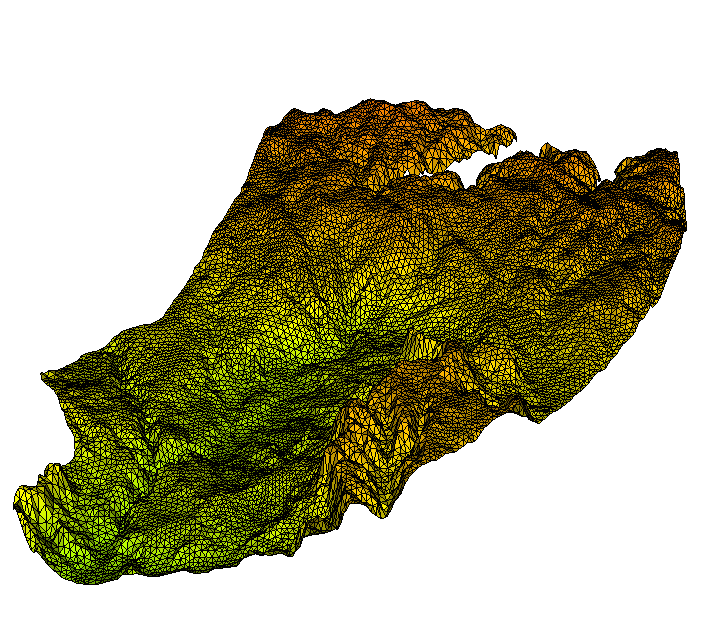
\includegraphics[width=0.3\linewidth]{AmmerSurface}\label{fig:AmmerSurface}}\enspace
\subfloat[Subsurface Layers]{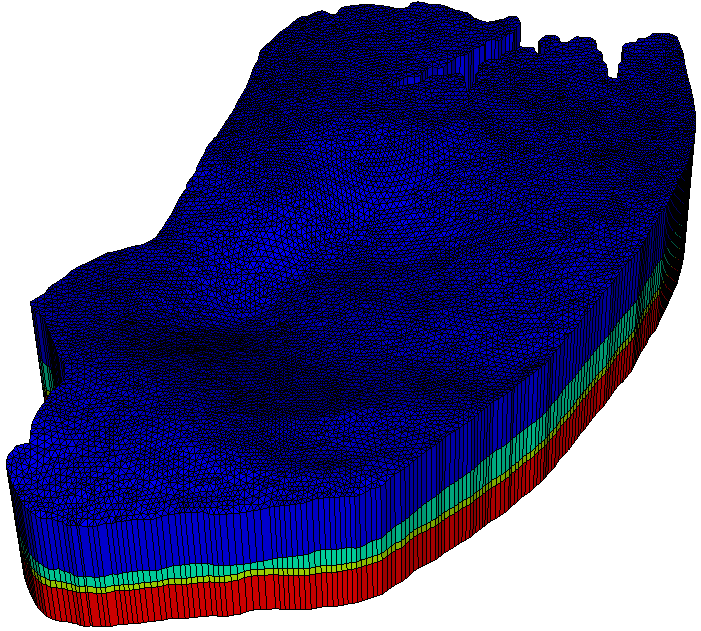
\includegraphics[width=0.3\linewidth]{AmmerSubsurface}\label{fig:AmmerSubsurface}}\enspace
\subfloat[Final Mesh]{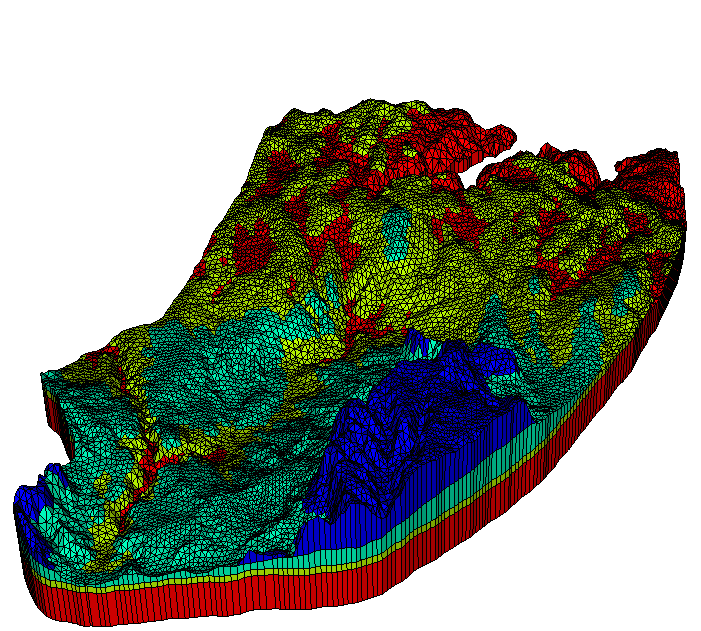
\includegraphics[width=0.3\linewidth]{AmmerFinal}\label{fig:AmmerFinal}}
\end{center}
\caption{Mapping meshes based on raster files: A surface mesh is extruded and four layers are added. These subsurface layers are mapped according to elevation models. In a final step the subsurface model is intersected with the terrain model.}
\label{fig:RasterMapping}
\end{figure}

For meshes containing only 2D elements there is also an option ``Remove mesh nodes at NoData values''. Per default this option is switched off as the correctness of the result is depending on the element size in these NoData locations.


\subsection{Analyse Mesh Quality}
\index{Mesh quality}

You can visualise the quality of a given mesh by right-clicking on the mesh in the respective Data View and selecting \cmd{Check Mesh Quality...}. This currently allows to choose between four implemented measurements for mesh element quality. The result of choosing any of these modes is a colour-codes overlay of the mesh where every element is assigned a quality in $[0,1]$. You can select this overlay in the visualisation pipeline and specify thresholds to select a certain range of quality and see which element fall into that range. \emph{(Note: You might need to manually set the correct scalar array for visualising mesh quality. The appropriate data can be chosen by selecting in ``C-Selection'' in the \cmd{Active Scalar} pull-down menu.}

\begin{figure}[tb]
\begin{center}
\subfloat[Edge Aspect Ratio]{\includegraphics[width=0.3\linewidth]{MshQualEdgeRatio}\label{fig:mshqual1}}\enspace
\subfloat[Element Area]{\includegraphics[width=0.3\linewidth]{MshQualArea}\label{fig:mshqual2}}\enspace
\subfloat[EquiAngle Skewness]{\includegraphics[width=0.3\linewidth]{MshQualEquiAngle}\label{fig:mshqual3}}
\end{center}
\caption{Examples for colour coded mesh quality measurements.} \label{fig:mshqual}
\end{figure}

The currently implemented measures are the following:
\begin{itemize}
\item \textbf{Aspect Ratio of Edge Length:} Analyses the ratio of shortest to longest edge of every element. Equilateral elements are often considered superior and better suited for FEM simulation, therefore these elements are rated ``1'' with their quality degrading with increasing differences in edge length. Each element is assigned the value of the highest ratio between any two of its edges. This is a good measure for triangle elements but might be not as good as others. See figure \ref{fig:mshqual1}.
\item \textbf{Area of 2D Elements:} Compares the area of all 2D elements (this includes the faces of 3D elements!) by assigned ``1'' to the element with the largest area and ``0'' to the element with the smallest area. See figure \ref{fig:mshqual2}.
\item \textbf{Volume of 3D Elements:} As with the area-criterion, this measure compares the volume of 3D mesh elements. 2D elements are ignored when this option is selected.
\item \textbf{Angles between Adjacent Edges:} Calculates the maximum deviation of an angle between any two adjacent edges of the element from the ``optimum'' angle, i.e. the angle of an equiangular element. This optimum angle is $90\degree$ for triangles or tetrahedra and $90\degree$ for quadrilateral or hexahedral elements. This measurement is called \emph{EquiAngle Skewness} and given by
    \begin{equation}
    s = \max\left[\frac{\theta_{max}-\theta_{opt}}{180-\theta_{opt}},\frac{\theta_{opt}-\theta_{min}}{\theta_{opt}}\right]
    \end{equation}
    where $\theta_{max}$ is the maximum angle between any two edges found in the element, $\theta_{min}$ is the minimum angle and $\theta_{opt}$ is the optimum angle.
    See figure \ref{fig:mshqual3}.
\end{itemize}

The quality measure best suited for a given mesh might depend on the process you want to simulate using this mesh. For instance, processes such as groundwater recharge consist mainly of layered flows, meaning that large differences between horizontal and vertical element surfaces might have no effect on a correct result. The simulation of mass transport processes explicitly requires a fine mesh resolution in vertical direction to ensure a stable solution.

\subsection{Changing Material Groups}
\index{Changing material groups}

Each element in a mesh is assigned a non-negative integer that specifies a material group this element belongs to. These material groups can be arbitrarily assigned. For instance, a mesh containing only two groups could name these groups ``17'' and ``98'' or use some different, arbitrary IDs. By right-clicking on a mesh and selecting \cmd{Edit Material Groups...} it is possible the change the ID of one or more groups or to merge groups.

The two basic options are ``Condense material groups to smallest possible range'' and ``Replace material group value''. The first option will rename all material groups such that the group with the smallest ID will be assigned $0$, the group with the second-smallest ID will be assigned $1$, and so on. In a mesh with $10$ different material groups the largest existing ID will be $9$ after processing the mesh.

The second option allows to specifically rename the ID of any group from the current value $A$ to any new value $B$. If $B$ already exists, the programme will give a warning and ask the user if the renaming process should really be started, thus merging groups $A$ and $B$.

\section{Modelling Data}

\subsection{Creating Processes}
\index{Creating processes}

It is possible to add processes to the workflow in the Modelling-tab by pressing the \cmd{Add process...}-button. A dialogue will open that allows to select a process type and an associated primary variable. As of version 5.2.07 this has no effect on output files except for boundary conditions being grouped under these processes and being removed upon removing the process (via right-click \cmd{Remove process}).

\subsection{Creating FEM Conditions}
\index{Creating FEM conditions}
\index{Creating boundary conditions}

It is possible to create FEM conditions based on geometric objects. By right-clicking on the respective point, polyline or surface and selecting \cmd{Set as FEM condition...} a setup dialogue will open (Fig. \ref{fig:CondSetupDlg}). Here, it can be specified for which process and primary variable the condition should be used and if it should be a boundary condition, a source term or an initial condition. Based on the geometrical object type and the selection of the condition type a number of distribution types will be available. For example, points as boundary conditions can only have \emph{Constant (Dirichlet)} distribution; lines as source terms can have \emph{Constant (Neumann)} or \emph{Linear (Neumann)} distribution, etc.

\begin{figure}[tb]
\begin{center}
\subfloat[FEM Condition Setup]{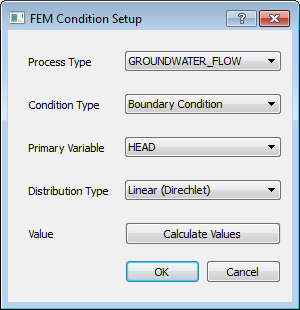
\includegraphics[height=4.0cm]{dlg_cond_setup}\label{fig:CondSetupDlg}}\enspace
\subfloat[Linear]{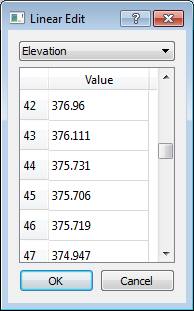
\includegraphics[height=4.0cm]{dlg_lin_dist}\label{fig:LinearDlg}}\enspace
\subfloat[Direct]{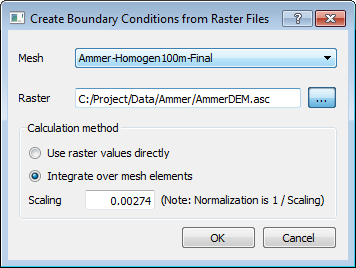
\includegraphics[height=4.0cm]{dlg_direct_dist}\label{fig:DirectDlg}}
\end{center}
\caption{Dialogues for creating of FEM Conditions.} \label{fig:CondSetup}
\end{figure}

While the assignment of values is easy for \emph{constant} distributions, it an get quite complex for \emph{linear} or \emph{direct} distributions. The FEM Condition Setup Dialogue will therefore contain a button ``Calculate Values'' instead of a textfield. Upon pressing this button a (different) dialogue will open to configure the values. For \emph{linear} distributions a table is displayed where for each point of the line a value can be inserted (Fig. \ref{fig:LinearDlg}). Conditions are only actually set up between points with given values. As an alternative it is possible to automatically insert the elevation (z-Coordinate) for each point of the line. For \emph{direct} distributions the dialogue will require to specify a raster file from which values are read for direct assignment to mesh nodes (Fig. \ref{fig:DirectDlg}). The user can select between a 1:1 assignment or a surface integration based on the area of the mesh elements the respective node is part of. In this case it is also possible to specify a scaling value to compensate for data files with different units of measurement.

For polylines or surfaces it is also possible to assign the conditions not directly on the geometric objects but instead on all points compromising the object. For example, a polyline consisting of 50 points can be either assigned one boundary conditions with a linear distribution or 50 boundary conditions on the respective points, each of which has a constant value.

Once created, FEM conditions can be saved by right-clicking associated process in the ``Modelling'' tab and selecting \cmd{Save FEM conditions...}. The user can specify the file format (XML or ASCII) and the type of conditions that should be written (boundary conditions, initial conditions, source terms or all of them).

\subsection{Changing FEM Conditions}
\index{Changing FEM conditions}

Conditions loaded into the \ogs Data Explorer can be edited simply by right-clicking the respective geometric object in the ``Modelling'' tab and selecting \cmd{Edit condition}. This will once again open the FEM Condition Setup Dialogue that is also used for creating conditions. For existing conditions the appropriate values will already have been selected and can now be changed. Changes in the corresponding files will only be written once the user actively saves these files again via \cmd{Save FEM Conditions...}



\chapter{Visualisation}

\section{Visualisation Properties}
\index{Visualisation settings}

You can change some properties of the render window by clicking \cmd{Settings\ra} \cmd{Visualisation Settings...}. The dialogue that opens allows you to change the background colour of the render window as well as some small changes concerning the illumination of the scene.

For any rendered scene a light source has to be specified (basically the equivalent to the sun or a lamp in the room). Per default this light source is identical with the viewer, i.e. the light source always illuminated the part of an object in the render window that can be seen by the user. In some cases this illumination is not enough, though, and certain parts of a rendered object may be shrouded in darkness. Therefore it is possible to switch on additional light sources above and below the object to ensure a full illumination of the scene.

A global superelevation\index{Superelevation} factor can be applied to all root objects in the visualisation pipeline. This overwrites all previously set superelevation factors. This is especially useful when dealing with a large number of files, all of which should be assigned the same superelevation factor (e.g. when using \ogs projects, see section \ref{nativefileformats}).

Per default on loading new data the 3D view is adapted to show the entire scene. This can be switched of by unchecking the ``Reset view on load'' option. This might be useful when making a series of screenshots with the exact same point of view.

Finally, it is possible to switch on backface culling. This will result in rendering only triangles with normals directed towards the camera/observer. This improves rendering speed and may be useful for finding false ordered primitives
\section{General Visualisation Options}
\label{genvisoptions}

For each object in the visualisation pipeline there a number of parameters that can be changed to make the object more easily distinguishable or to convey information contained in the data.

\begin{figure}[tb]
\begin{center}
\subfloat[Solid Color]{\includegraphics[width=0.3\linewidth]{colour-solid}\label{colour-solid}}\enspace
\subfloat[Default colour table]{\includegraphics[width=0.3\linewidth]{colour-default}\label{colour-default}}\enspace
\subfloat[User-defined colours]{\includegraphics[width=0.3\linewidth]{colour-user}\label{colour-user}}
\end{center}
\caption{Each object is assigned a random solid colour as well as a default colour table based on a temperature scale (from blue to red). The solid colour can be adjusted via the ``Diffuse Color''-option (see section \ref{genvisoptions}), the colour table can be adjusted by loading a user-defined *.xml file via the ``Add color table...''-option (see section \ref{specvisoptions}).} \label{fig:colours}
\end{figure}

In detail these parameters are:

\begin{itemize}
\item \textbf{Diffuse Color:}\index{Changing Colour} Each item is assigned a colour which is used for rendering the object in 3D space. This colour can be changed here (see figure \ref{colour-solid}).
\item \textbf{Active Scalar:}\index{Changing scalar values} Each visualisation object has an assigned colour which is used in the rendering process (see above). However, some data sets contain additional information (e.g. material groups for meshes, concentration of chemical substances, etc.). This information can be selected here and is then employed in the rendering of object in the render window (see figure \ref{colour-default}).
\item \textbf{Visible Edges:}\index{Edges} Some objects (such as meshes) are composed of a combination of lines (edges) and surfaces. While the colour of the surfaces can be set using the \emph{Diffuse Color}-button, the colour of the edges can be changed here. Furthermore the rendering of edges can be switched off by unchecking the box next this option.
\item \textbf{Opacity:}\index{Opacity}\index{Transparency} Determines if an object appears to be transparent or not.
\item \textbf{Scaling Factor:}\index{Scaling} Super-elevates the data by the given factor. This makes it much more easy to recognise differences in height.
\item \textbf{Translation:}\index{Translation} Any data set can be moved in x, y or z-dimension so data sets can be set in relation to each other for comparison or layered visualisation.
\end{itemize}

In addition, there are a number of visualisation options applied to the whole scene. These are activated via buttons above the render window and include

\begin{itemize}
\item \textbf{Show All:} Rotates the scene into the (x,y)-plane and zooms to a point where the whole scene is visible.
\item \textbf{Zoom:}\index{Zoom} If this button is activated pressing the left mouse button will draw a square into which the programme will zoom upon releasing the button. If the button is deactivated again, the left mouse button will again rotate the scene.
\item \textbf{Highlight:}\index{Bounding Box} If this button is activated, a bounding box will be drawn for the object currently selected in the Visualization Pipeline.
\item \textbf{Ortho:}\index{Projection}\index{Orthographic Projection}\index{Perspective Projection} This button causes a orthographic projection of the scene (i.e. objects in the distance will \emph{not} appear smaller). If it is deactivated again, the projection will use perspective again.
\end{itemize}


\section{Object-specific Visualisation Options}
\label{specvisoptions}

There are a number of options that are available only for certain types of data. These options can be selected by right-clicking on an item in the visualisation pipeline.

\begin{itemize}
\item \textbf{Add filter...:} Allows to apply a filter to the current objects. For details on that option see section \ref{filters}.
\item \textbf{Add color table...:}\index{Colour lookup tables} Allows you to assign a specific colour table to the currently selected scalar array (see figure \ref{colour-user}). The colour table is loaded from a *.xml-file and has the same format as ParaView\footnote{ParaView is an open-source data analysis and visualisation application for VTK data. It can be downloaded at \url{http://www.paraview.org/}}.\index{ParaView}\\
    This option is available for all objects, although for image data it is not available via right-click but needs to be called as a filter (see section \ref{filters}) lookup tables and can therefore be created or edited using this software.
\item \textbf{Convert to Mesh...:} Allows to convert an object of the VTK-data type ``Unstructured Grid'' to be converted into an \ogs mesh. Objects of that type are basically meshes that are contained in different data structure than ``normal'' \ogs meshes. Therefore, this specifically allows the conversion of imported VTK-files to \ogs meshes.\\
    This option is available for all objects of type ``VTK\_UN\-STRUCT\-URED\_GRID'' (i.e. all mesh objects).
\item \textbf{Convert Image to Mesh...:} Generates an \ogs mesh based on a given raster file. See figure \ref{Filter-Img4}. For more information, see section \ref{meshraster}. This options is only available for image data (i.e. raster files).
\item \textbf{Export to VTK:}\index{VTK export} All objects displayed the render window are technically VTK-objects. Choosing this option saves these objects in VTK-format to a file. They can then be used in any software supporting this format (e.g. Paraview).
\item \textbf{Export to OpenSG:}\index{OpenSG export} Converts objects into OpenSG format (*.osg). This is another open source graphics format. It is also the format used by the UFZ VisLab. Specifically, this also implies that \emph{anything} that can be visualised in \ogs can also be exported to OpenSG and be presented in the VisLab.
\end{itemize}

\section{Applying Filters for Visualisation}
\label{filters}

In contrast to the options detailed in the previous section, filters are a manipulation of the actual graphics object to enhance, reduce or deform certain aspects of these objects for imparting information that might not be superficial\footnote{One might argue that this definition also holds true for the assignment of specific color tables which is accessed via right-click on an object. This inconsistency originates in the data structures the objects are stored in and in defining an easy-to-use workflow for using this functionality.}.

To apply a filter, right-click on an object in the visualisation pipeline and select \cmd{Add filter...}.\index{Adding filters}\index{Filter} A dialogue will pop up which lets you select one of a number of available filters. As before, filters will only be displayed for objects they can be applied to. However, this does not mean that it makes sense to apply any filter to any object where it can be applied. Also note, that it is possible (and sometimes useful) to apply filters to filters to extract certain information bit by bit.
%
\begin{figure}[tb]
\begin{center}
\subfloat[Raster data]{\includegraphics[width=0.4\linewidth]{Filter-Img1}\label{Filter-Img1}}\enspace
\subfloat[Apply lookup table to image]{\includegraphics[width=0.4\linewidth]{Filter-Img2}\label{Filter-Img2}} \\
\subfloat[Image to bar chart]{\includegraphics[width=0.4\linewidth]{Filter-Img3}\label{Filter-Img3}}\enspace
\subfloat[Convert Image to Mesh]{\includegraphics[width=0.4\linewidth]{Filter-Img4}\label{Filter-Img4}}
\end{center}
\caption{\ogs functionality applicable to image-/raster-data.} \label{fig:filter:raster}
\end{figure}
%
All available filters will be detailed in the following.

\subsubsection{Apply lookup table to image}
\bstart{Applicable to:} Image Data
\index{Colour lookup tables}

\bstart{Effect:} Applies a color table to images. The color table can be loaded from a *.xml-file. If no file is specified, a default color table is automatically generated, replacing grey values with a temperature scale (i.e. dark colours are blue, light colours are red). This results in an image where certain gradients are much better discernable. See figure \ref{Filter-Img2}.

\bstart{Remarks:} \emph{This is similar to applying a pre-defined colour table to a geometry- or mesh object. The implementation as a filter for images is based on the very different structure of image objects in the graphics library VTK which is used for visualisation.}

\begin{figure}[tb]
\begin{center}
\subfloat[Geometry Data]{\includegraphics[width=0.4\linewidth]{Filter-Poly1}\label{Filter-Poly1}}\enspace
\subfloat[Points to Spheres]{\includegraphics[width=0.4\linewidth]{Filter-Poly2}\label{Filter-Poly2}} \\
\subfloat[Lines to tubes]{\includegraphics[width=0.4\linewidth]{Filter-Poly3}\label{Filter-Poly3}}\enspace
\subfloat[Extract cells by threshold]{\includegraphics[width=0.4\linewidth]{Filter-Poly4}\label{Filter-Poly4}}
\end{center}
\caption{\ogs functionality applicable to geometry data. In figure \ref{Filter-Poly2} ground water stations in the area have been emphasised. In figure \ref{Filter-Poly4} a threshold filter has been applied to the tube-filtered data from figure \ref{Filter-Poly3} to select only the river network of the depicted area from the geometric data.} \label{fig:filter:poly}
\end{figure}

\subsubsection{Apply texture to surface}
\index{Textures}\index{Raster files}\index{Raster files}\index{NetCDF files}
\bstart{Applicable to:} Surfaces, Meshes

\bstart{Effect:} Allows to map an image/raster on a surface or mesh. This might be additional information such as land use classes, precipitation, etc. Possible formats for loading textures include all supported raster formats as well as netCDF files (see \ref{Import File Formats}). An example is shown in figure \ref{Filter-Mesh4}.

\subsubsection{Elevation-based colouring}
\bstart{Applicable to:} Geometry, Meshes

\bstart{Effect: } Applies a colour to each point depending on the z-coordinate of that point, assuming that this denotes height in metres. The pre-defined colour scale starts with blue up to a height of $0$ metres (i.e. sea level), which is then slowly changing to green (150\,m) and yellow (450\,m) and then changing to red from then on. See figure \ref{Filter-Mesh2}.

\bstart{Remarks:} \emph{In theory these values can be changed. This is, however, currently not possible using the GUI.}

\begin{figure}[tb]
\begin{center}
\subfloat[Multilayered Mesh]{\includegraphics[width=0.4\linewidth]{Filter-Mesh1}\label{Filter-Mesh1}}\enspace
\subfloat[Elevation-based colouring]{\includegraphics[width=0.4\linewidth]{Filter-Mesh2}\label{Filter-Mesh2}} \\
\subfloat[Extract cells by threshold]{\includegraphics[width=0.4\linewidth]{Filter-Mesh3}\label{Filter-Mesh3}}\enspace
\subfloat[Apply texture to surface]{\includegraphics[width=0.4\linewidth]{Filter-Mesh4}\label{Filter-Mesh4}}
\end{center}
\caption{\ogs functionality applicable to meshes.} \label{fig:filter:mesh}
\end{figure}

\subsubsection{Extract cells by threshold}
\index{Threshold filter}
\bstart{Applicable to:} Lines, Surfaces, Meshes

\bstart{Effect:} Each line, surface and mesh layer has a unique ID which allows to assign different colours to different objects. This filter furthermore allows to select a range of objects which should be displayed while all other objects are blanked out. This way you can visualise only a specified stratigraphic layer or a certain polyline, etc. See figures \ref{Filter-Poly4} and \ref{Filter-Mesh3}. The filter is always applied to the currently selected scalar array. For instance, given a mesh containing scalar arrays for material group and groundwater head, this filter may be used to select a range of materials (e.g. only materials with IDs 5--7) or regions with a certain groundwater head (e.g. $\text{head}>7.2$).

\subsubsection{Generate contours based on scalar fields}
\index{Contour filter}
\bstart{Applicable to:} Meshes

\bstart{Effect:} Given a scalar field this filter will output contour lines of meshes containing 2D elements and contour surfaces for meshes containing 3D elements. The number of contours that should be displayed can be defined in the filter properties as well as the minimum and maximum value for the calculated contours. The chosen number of contours will that be calculated on the selected scalar field in equidistant intervals between the chosen minimum and maximum value. The colours of the contours are automatically chosen based on these scalar values.

\subsubsection{Image to bar chart}
\bstart{Applicable to:} Image Data

\bstart{Effect:} Each pixel is assigned a bar depending on the grey value of the pixel. Also, the colour changes of that bar changes according to its height. See figure \ref{Filter-Img3}.

\bstart{Remarks:} \emph{This filter takes a lot of time for large images as the result becomes very complex. The intention is to use it for low resolution raster data of phenomena such as precipitation, etc.}

\emph{This is a good example on the combination of the successive application of these filters. This one combines `Image to vertical lines', `Lines to tubes' and `Elevation-based colouring'.}

\subsubsection{Image to vertical lines}
\bstart{Applicable to:} Image Data

\bstart{Effect:} Plots vertical lines for every pixel of a raster with each line having a height depending on the raster's grey value.

\bstart{Remarks:} \emph{This is a filter that is needed for the correct application of other filters. It is probably not of much use on itself.}

\subsubsection{Lines to tubes}
\index{Tube filter}
\bstart{Applicable to:} Geometry, Observation sites

\bstart{Effect:} A geometric line has independent of the current zoom level always a thickness of $1$. This filter allows to assign a `real' thickness to line-objects that also changes according to the current zoom. See figure \ref{Filter-Poly3}.

\subsubsection{Points to spheres}
\index{Sphere filter}\index{Glyph Filter}
\bstart{Applicable to:} Geometry, Observation sites

\bstart{Effect:} A geometric point has independent of the current zoom level always a diameter of $1$. This filter allows to assign a `real' diameter to point-objects that also changes according to the current zoom. See figure \ref{Filter-Poly2}.

\subsubsection{Surface filter}
\index{Surface filter}
\bstart{Applicable to:} Meshes

\bstart{Effect:} Extracts the outer surface of a mesh.

\bstart{Remarks:} \emph{This is a filter that is needed for the correct application of other filters. It is probably not of much use on itself.}


%\include{ch05-workflows}

\appendix

\cleardoublepage
\addcontentsline{toc}{chapter}{Index}
\printindex

\cleardoublepage
\phantomsection
\addcontentsline{toc}{chapter}{Further Reading}

\begin{thebibliography}{}

\bibitem{ogs04}
Kalbacher T, Mettier R, et al.: Geometric modelling and object-oriented software concepts applied to a heterogeneous fractured network from the grimsel rock laboratory.
\emph{Comput Geosci,} \textbf{11(1):} 9--26 (2007)

\bibitem{ogs05}
OpenGeoSys -- scientific software for coupled processes in porous media,
\texttt{http://www.opengeosys.org}

\bibitem{ogs06}
OpenGeoSys-Wiki: Source code, current projects, presentations and much more. \texttt{https://svn.ufz.de/ogs/}

\bibitem{ogs07}
Rink K, Bilke L, Selle B, Kolditz O: User Guided Generation of Hydrological Models: Interface Design, Workflows and Concepts for an Extensible Software Framework. \emph{Proc. of 6th
Int Congress on Environmental Modelling and Software (iEMSs2012),} (2012)

\bibitem{ogs07}
Rink K, Fischer T, Kolditz O: Data Visualisation and Validation for Hydrological Models. \emph{Proc. of International Conference on Computer Graphics, Visualization, Computer Vision and Image Processing (CGVCVIP2011),} pages 169--176 (2011)

\bibitem{ogs09}
Rink K, Fischer T, Selle B, Kolditz O: A Data Exploration Framework for Validation and Setup of Hydrological Models.
\emph{Environ Earth Sci,} \textbf{69(2)} (2013) 
DOI: 10.1007/s12665-012-2030-3

\bibitem{ogs03}
Rink K, Kalbacher T, Kolditz O: Visual Data Exploration for Hydrological Analysis. \emph{Environ Earth Sci,} \textbf{65(5):} 1395--1403 (2012)

\bibitem{ogs01}
Wang W, Kolditz O: Object-oriented finite element analysis of thermo-hydro-mechanical (THM) problems in porous media.
\emph{Int J Numer Meth Engng,} \textbf{69:}162--201 (2007)

\bibitem{ogs02}
Wang W, Kosakowski G, Kolditz O: A parallel finite element scheme for thermo-hydro-mechanical (THM) coupled problems in porous media \emph{Comput Geosci,} \textbf{35(8):}1631--1641 (2009)

\end{thebibliography} 

\cleardoublepage

\end{document}
